\scanpage{62}
\[
C'_i\ \left\{\begin{aligned}
&H^i(U,F(m))=0\quad\text{pour }m\text{ grand}\quad(i>0\text{ donné})\\
&\Updownarrow\\
&\underline H^{i+1}_Z(F)=0\quad\text{i.e.}\quad H^{i+1}_z(F_{\unsure{z|c}})=0\quad\text{pr }z\in Z\\
&\Updownarrow\\
&R^i g_*(F)=0
\end{aligned}\right.
\]
\[
\deleted{\unsure{\Updownarrow|\Downarrow}}\Downarrow
\]
\[
C_n\ \left\{\begin{aligned}
&H^i(U,F(m))=0\quad\text{pr }m\text{ grd,}\qquad0<i\leq n\\
&\hspace{16em}(n\geq1\text{ donné})\\
&\Updownarrow\\
&\deleted{H^i}\ [\text{à supposer que } F=g_*(F|U)]\quad\operatorname{prof}_z F>n+1\\
&\hspace{16em}\text{pr }z\in Z
\end{aligned}\right.
\]
Les conditions $C$ sont les seules qui exigent quelque chose sur la profondeur en les $z\in Z=X-U$ ..... et non seulement aux pts de $U$.

\figure{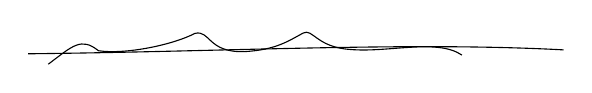
\begin{tikzpicture}[x=.85cm,y=.55cm]
\draw (0,0) .. controls (3,.05) and (5.7,.28) .. (8,.09);
\draw (.30,-.24) .. controls (.67,.19) and (.79,.39) .. (1.05,.07)
 .. controls (1.45,-.02) and (2.15,.20) .. (2.49,.47)
 .. controls (2.72,.56) and (2.68,.02) .. (3.23,.05)
 .. controls (3.70,.09) and (3.88,.29) .. (4.11,.48)
 .. controls (4.25,.59) and (4.31,.15) .. (4.81,.10)
 .. controls (5.38,.02) and (6.11,.36) .. (6.48,-.03);
\end{tikzpicture}}
% archive sheet number: 61
